%!TEX root = ../main.tex

\chapter{Response of an event-based camera\label{chap:response}}

\section{Equipment}

The event-based camera used in this work is the model EVK4\footnote{Prophesee EVK4 website: \url{https://www.prophesee.ai/event-camera-evk4/}.}, manufactured by Prophesee. The camera has a resolution of
$1280 \times 720$ pixels, with a maximum frame rate equivalent of 10k FPS and a dynamic range of 120 dB.
A fish eye lens with an inbuilt UV filter was used during the measurements to target the specific wavelength of the LEDs
that are used on the UAVs. The UAV used for measurements was a unit from the MRS UVDAR system, with UV \ac{LED} light sources, mounted at each arm of the UAV, which are used for localization and communication purposes.
Both can be seen in \reffig{fig:uavcam}.

\begin{figure}[H]
	\centering
	\subfloat[The event-based camera EVK4 from Prophesee with a fish eye lens.] {
	  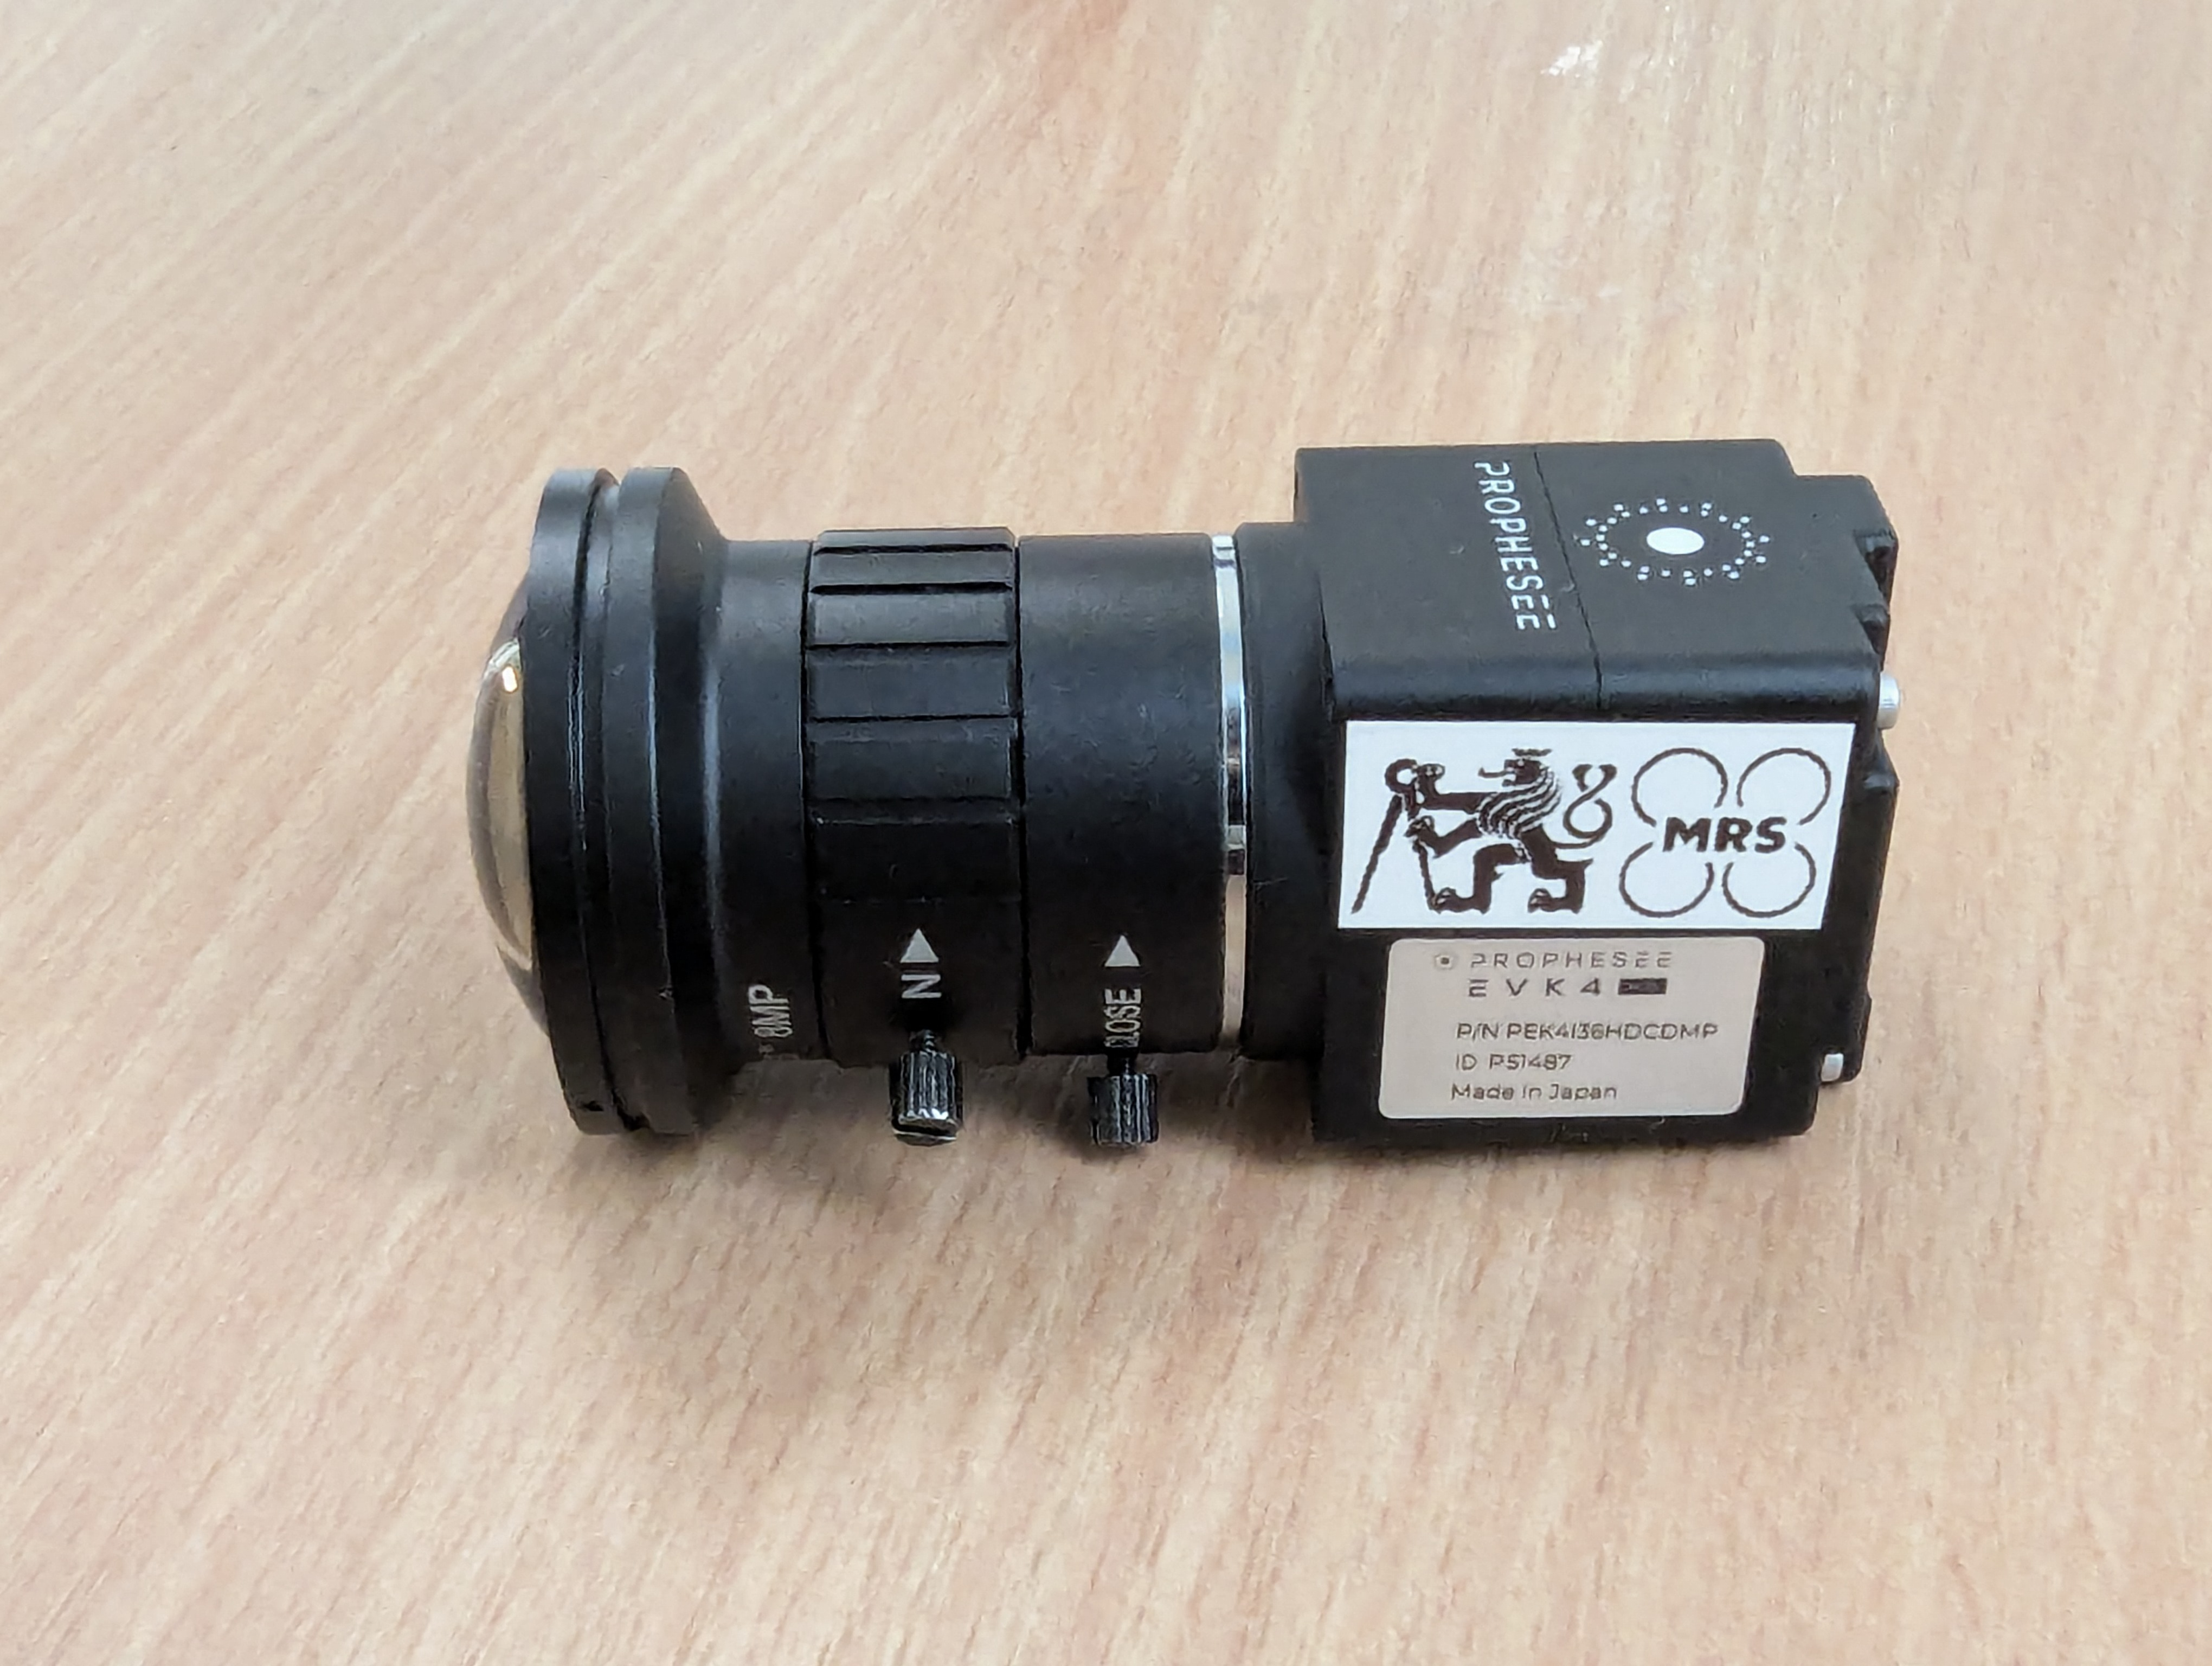
\includegraphics[width=0.5\textwidth]{./fig/photos/evk4.jpg}
	  \label{fig:evk4}
	}
	\subfloat[MRS UVDAR UAV unit] {
	  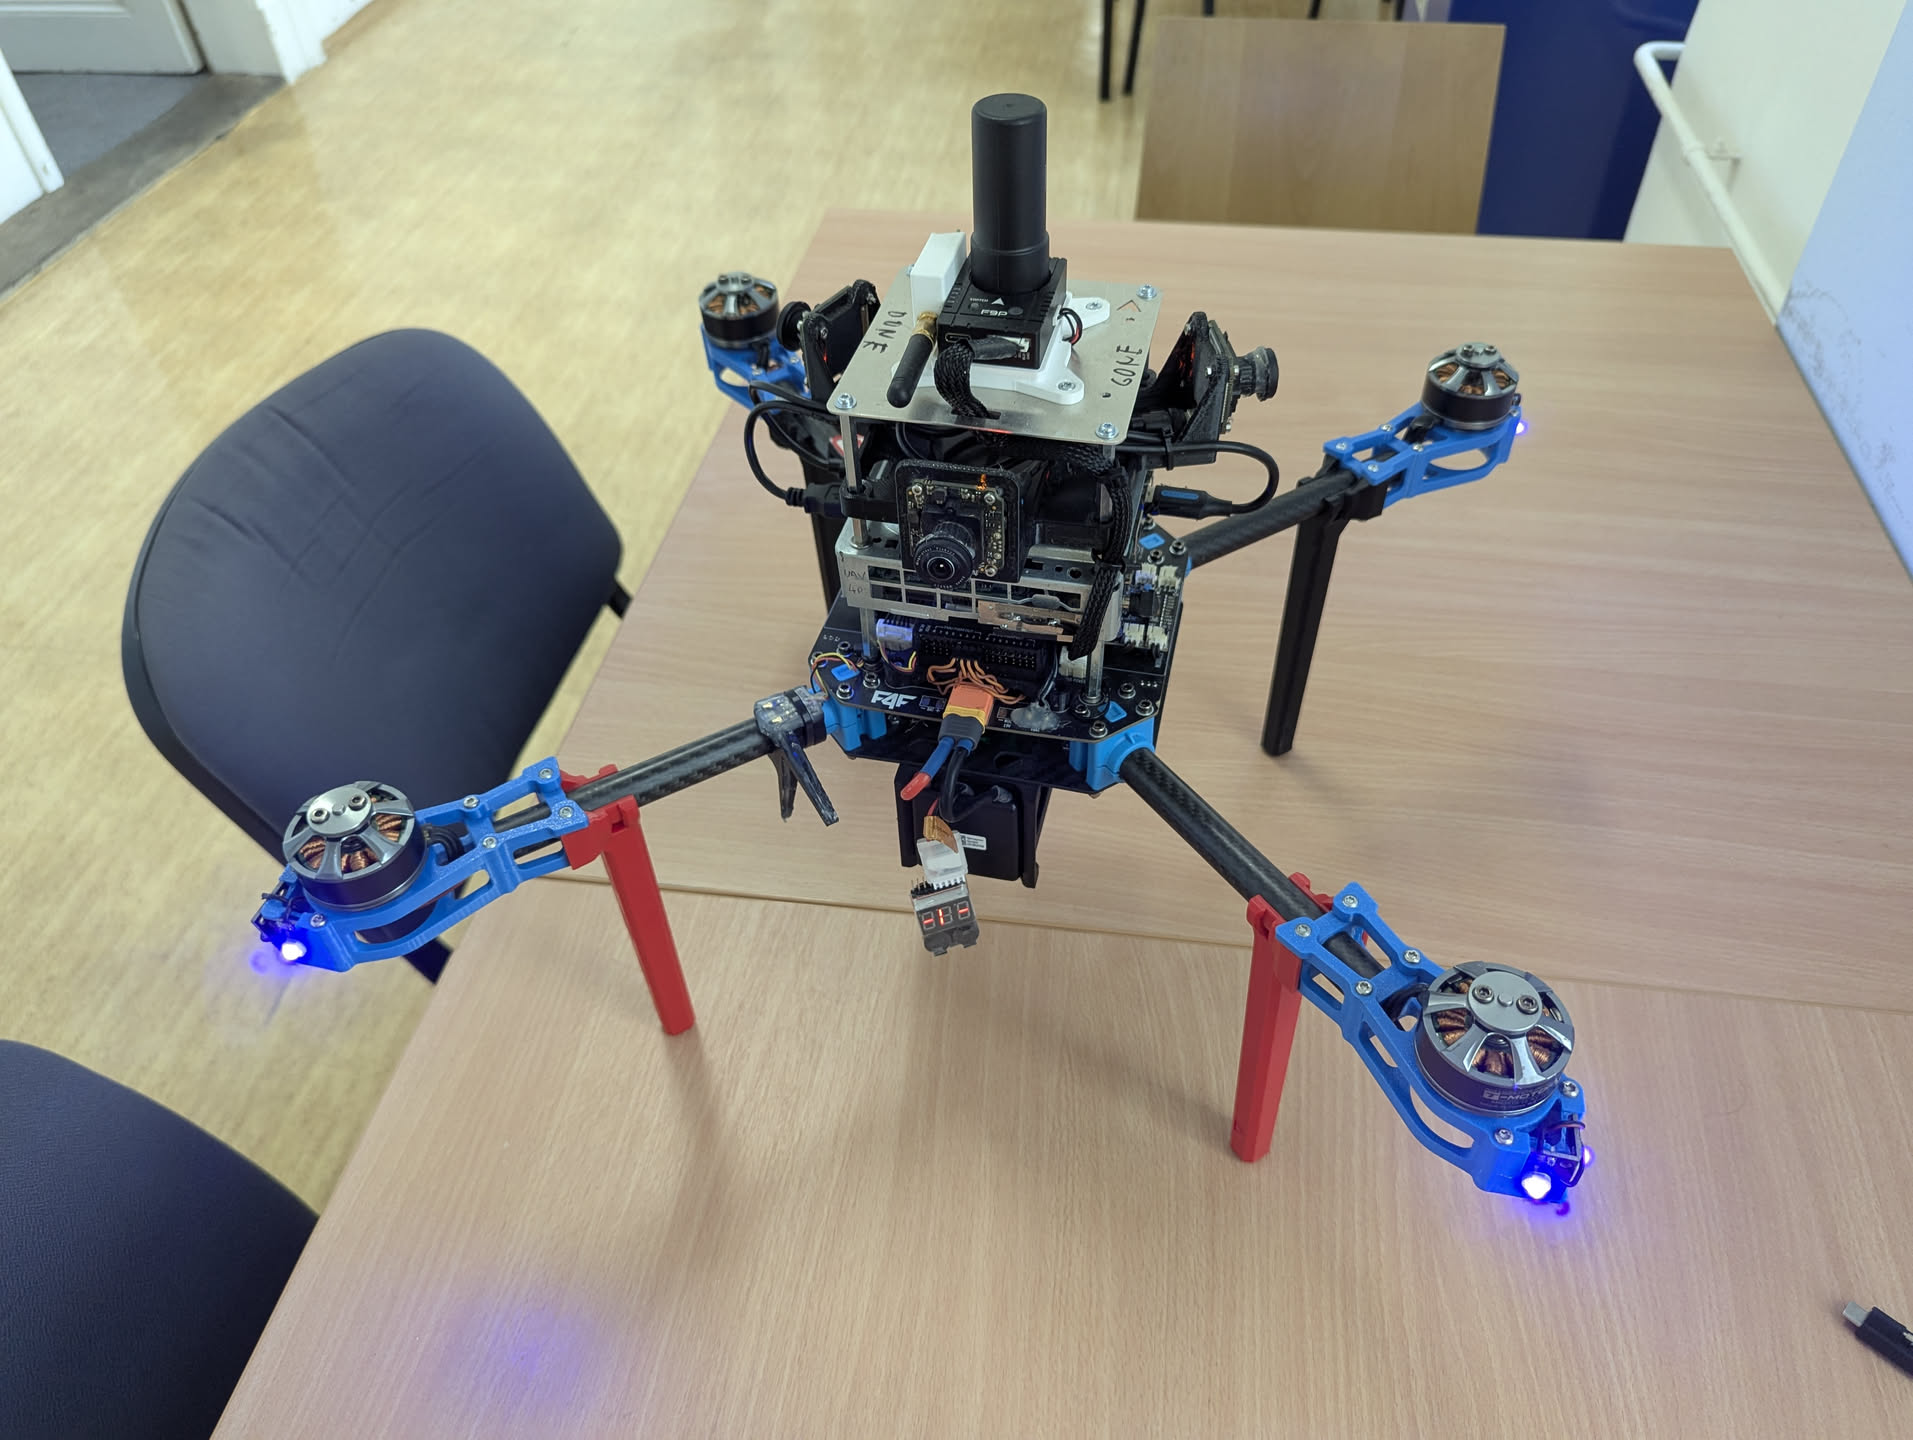
\includegraphics[width=0.5\textwidth]{./fig/photos/uav1.jpeg}
	  \label{fig:uav1}
	}
	\caption{
  An event-based camera with a fish eye lens can be seen on \reffig{fig:evk4}, which was used to measure the UV LEDs mounted on the UAV unit from the MRS UVDAR system as seen on \reffig{fig:uav1}.
  }
	\label{fig:uavcam}
\end{figure}

The camera data has been obtained using the Metavision Studio software, which records the data in \texttt{.raw} format.
The data is then processed later using various functions from the Metavision SDK\footnote{Metavision SDK Docs: \url{https://docs.prophesee.ai/stable/index.html}},
which has C++ or Python API. In this work, the Python API has been used.

\section{Data collection}

The data have been collected on several occasions by measuring a stationary UAV at various distances and rotations from the camera.
Each UAV is equipped with 8 UV LEDs, with 2 LEDs on each arm of the UAV. Each of the LEDs can be individually controlled
and can be set to various sequences of blinking, and a common modulation frequency can be set for all LEDs.

\subsection{Initial measurements}

The initial measurements were made by securing the event camera on a tripod and placing the UAV at distances ranging from
$0.5$ to $2.5$ meters. The LEDs were set to blink at a frequency in the range of $1$ to $30$ kHz. No \ac{ROI} was set
and the whole visible area was recorded during the testing.

This first experiment proved to be rather inefficient as the LEDs need to be isolated from each other's influence, which
was not done properly at this time. This problem is solvable in the post-processing, by filtering out the events
by using an ROI filter (it is possible to filter the events by finding bounding boxes
that encapsulate light sources, but on a more complex scene this approach becomes relatively hard).
The other issue turned out to be the reflections of surrounding objects (as seen in \reffig{fig:meas1}), which caused
another source of unwanted events in the recording, which may in turn confuse some blob detection methods.

\begin{figure}[H]
	\centering
	\subfloat[An event-camera view of the UAV with UV LEDs.] {
	  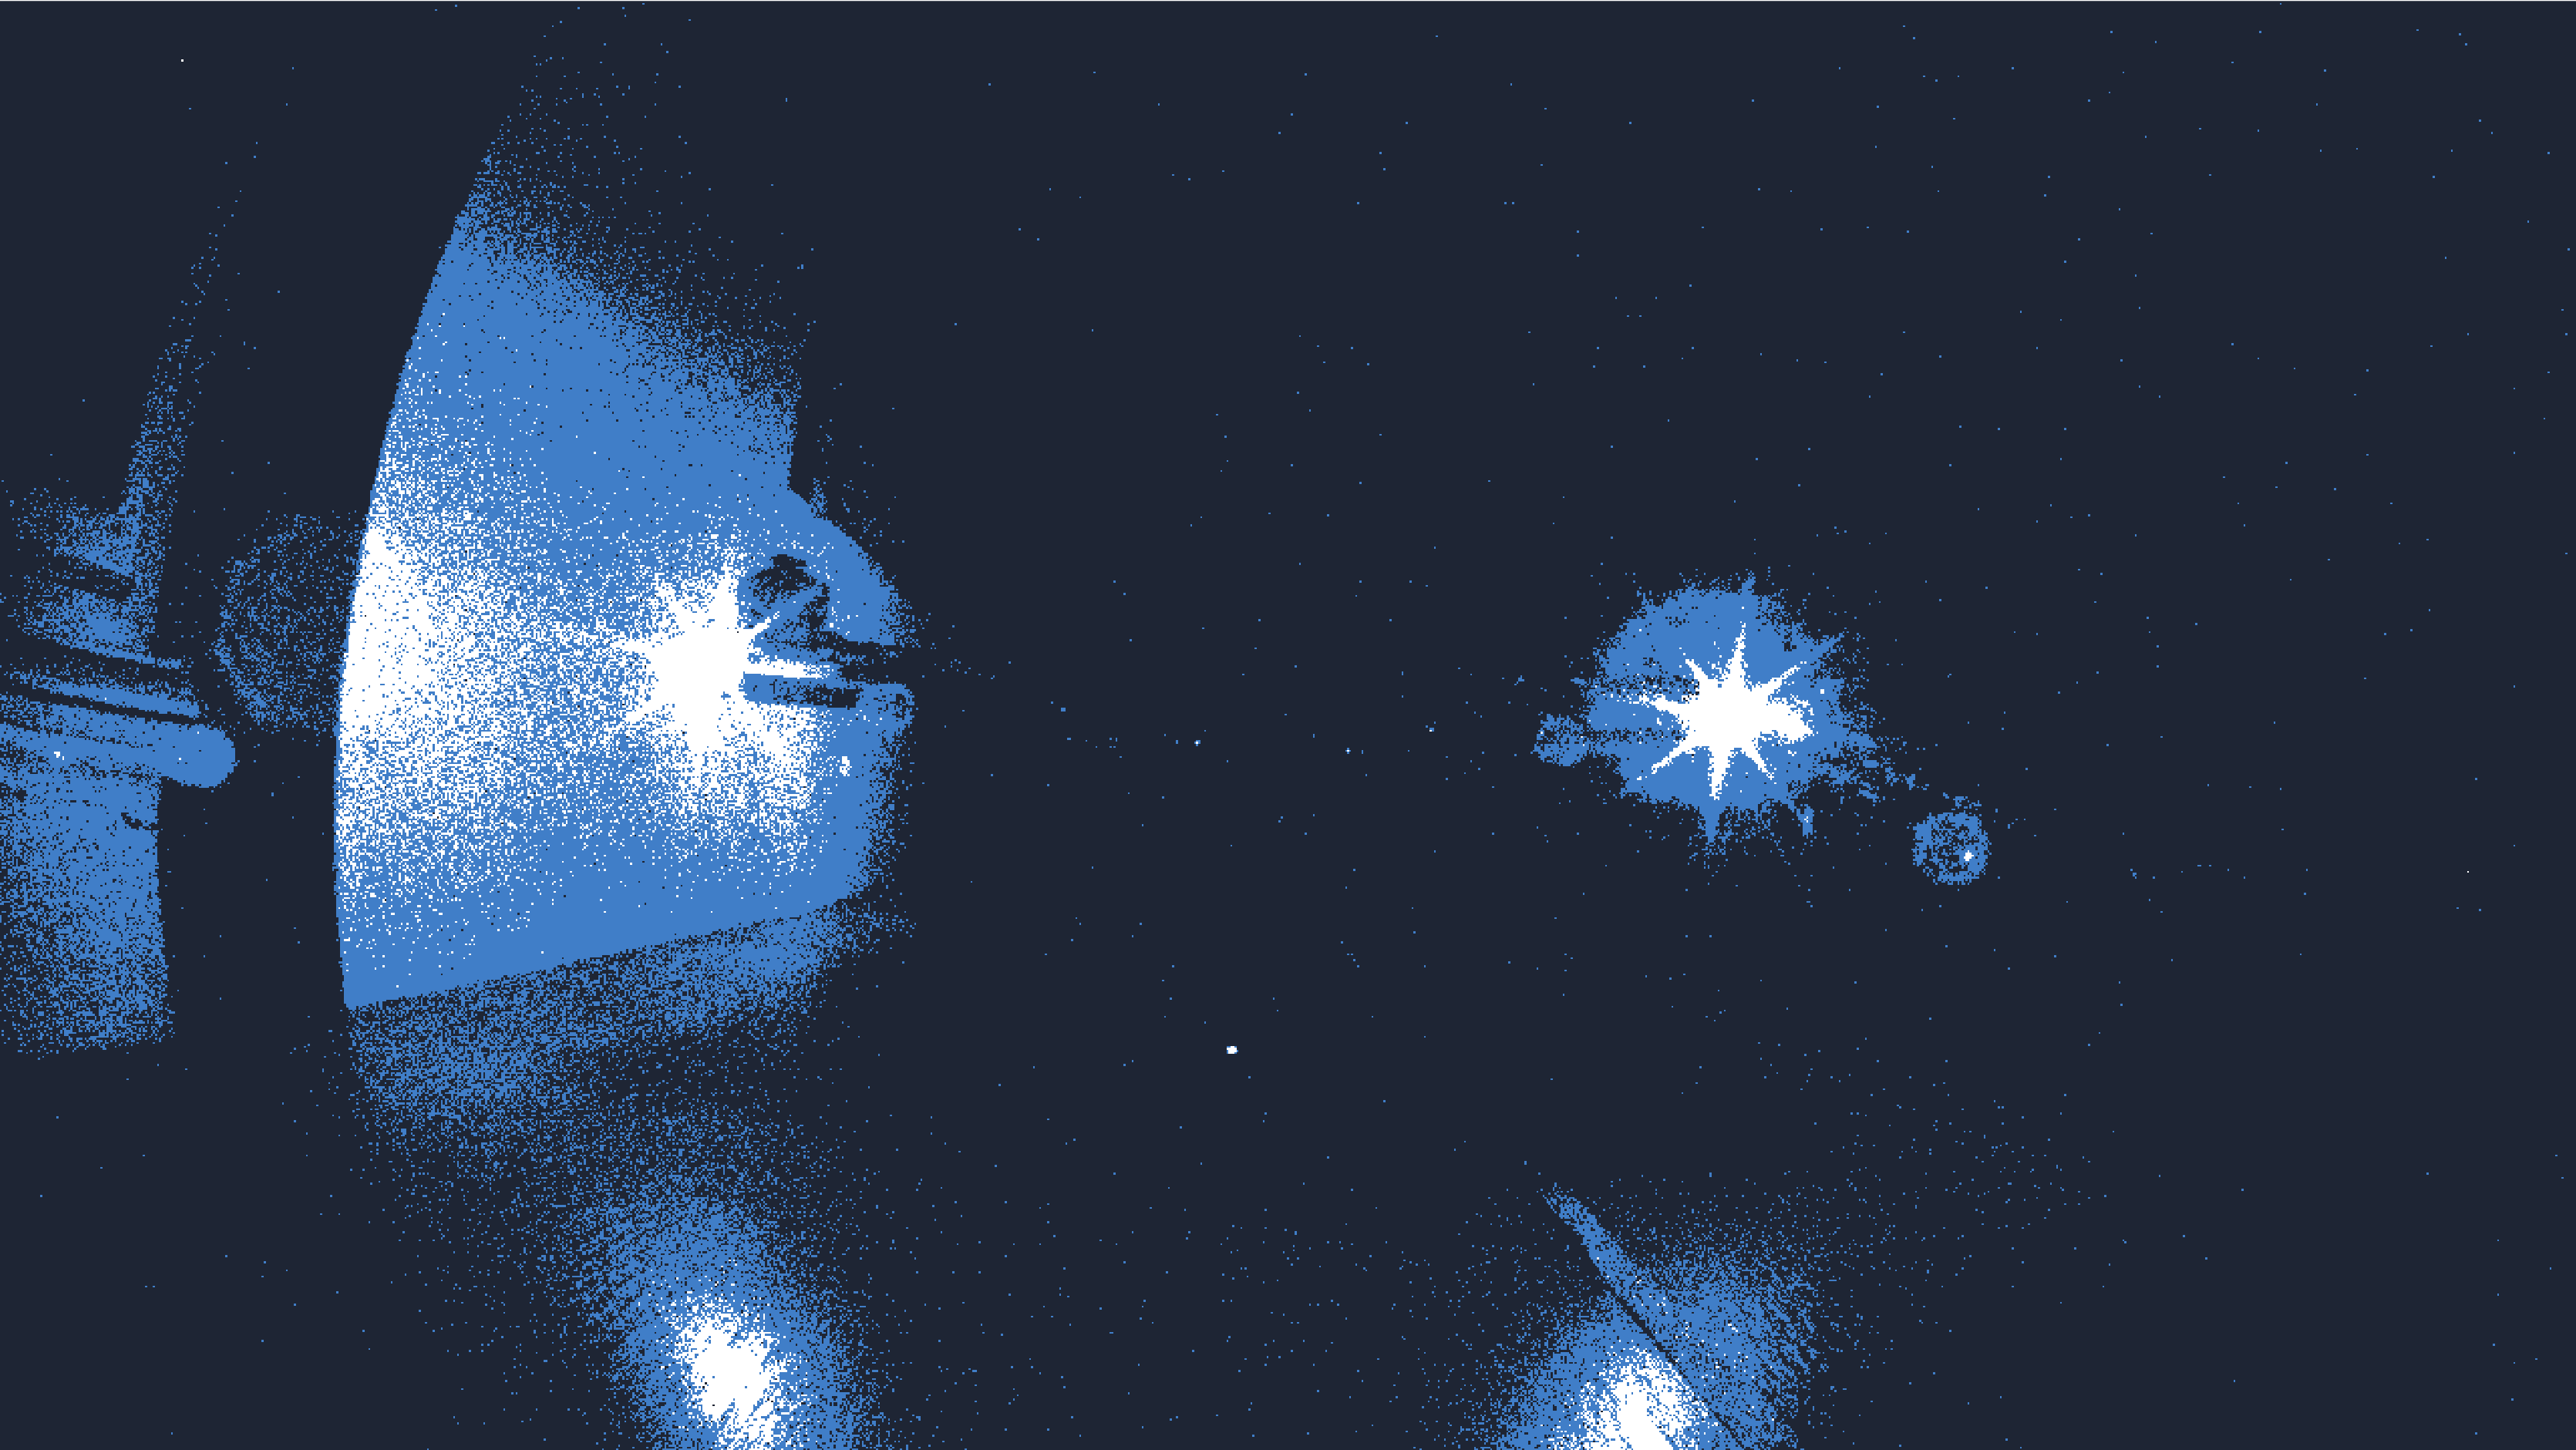
\includegraphics[width=0.5\textwidth]{./fig/photos/meas1.png}
	  \label{fig:meas1_e}
	}
	\subfloat[View of the experiment setup.] {
	  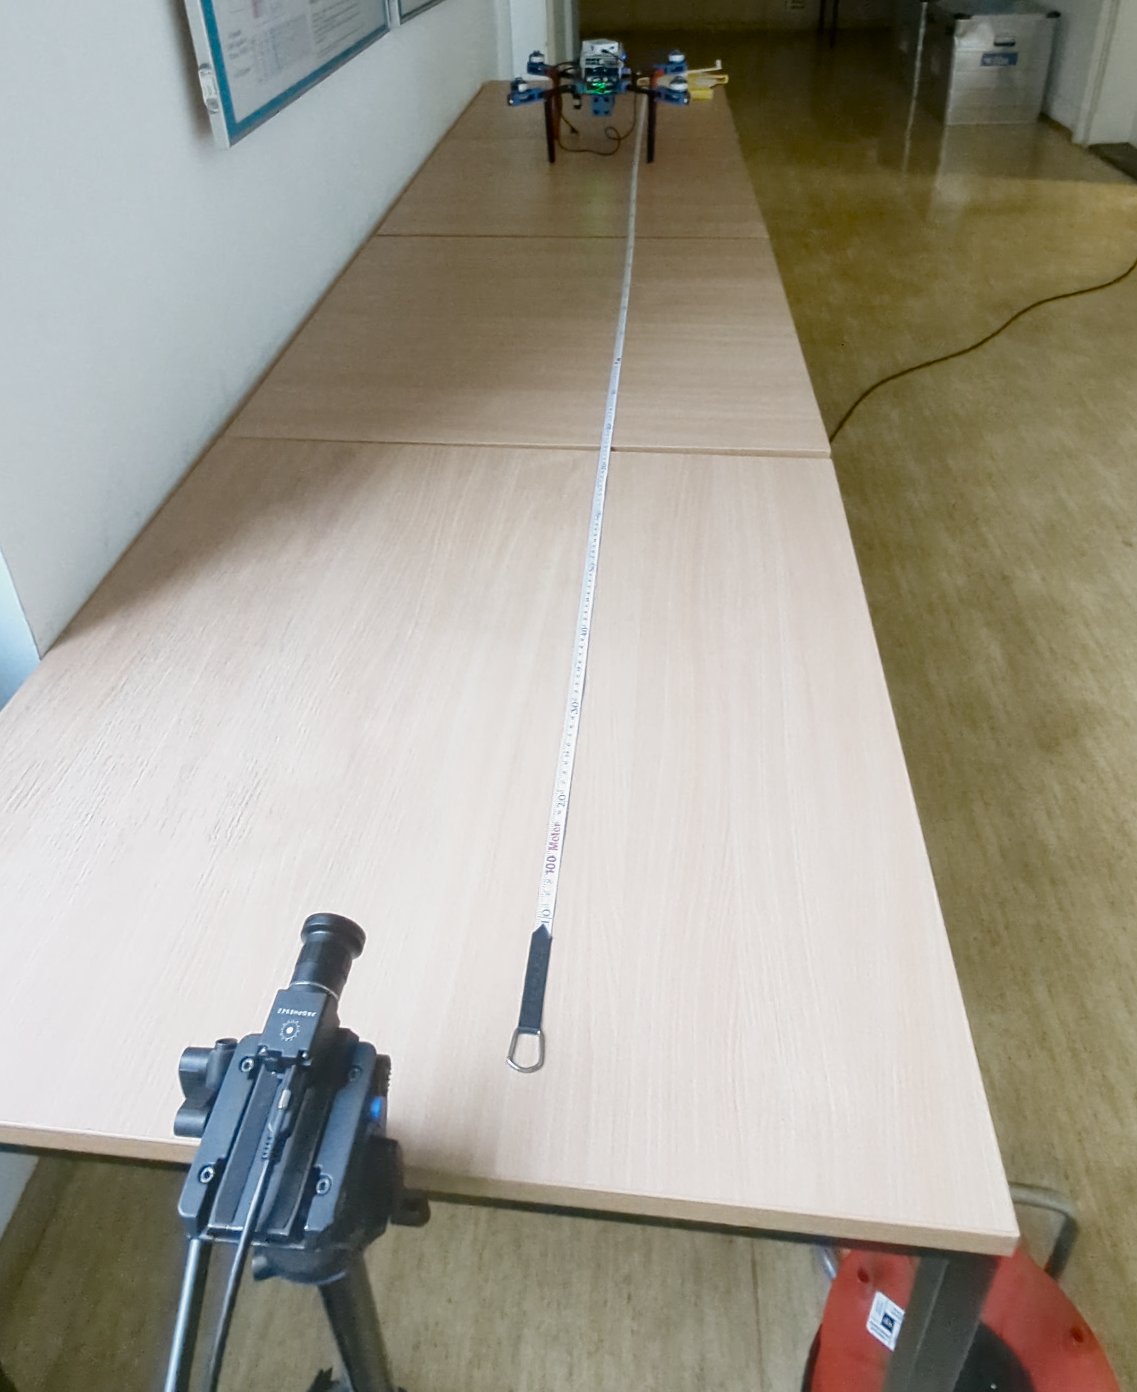
\includegraphics[width=0.5\textwidth]{./fig/photos/meas1_c.png}
	  \label{fig:meas1_c}
	}
	\caption{
  The setup for measuring the event-camera response with a EVK4 camera. Visible reflections from a wall can be seen on \reffig{fig:meas1}. The setup is shown on \reffig{fig:meas1_c}.
  }
	\label{fig:meas1}
\end{figure}


\subsection{Distance - frequency influence}

In the following measurements, we consider only one source of light as the whole end of the arm of the UAV (with 2 UV LEDs). Other arm light sources were turned off during the measurements.
Measurements were done on areas isolated by ROI filter directly in Metavision Studio, events were collected only on one select area around the light source, with the
rest of the events being discarded.
This time, the position of the UAV was fixed relative to the camera on a blank background. The camera was placed on a tripod
and moved in increments of $0.2$ meters, starting from $1$ meter and ending at $3$ meters, with additional measurements made
at $4$ and $5$ meters.
The frequency range of the LED modulation was set in a range of $10$ Hz to $30$ kHz, with the blinking sequence set to \texttt{0, 1}.

\subsection{Rotation angle influence}

In addition to distance and frequency influence, the rotation angle influence also needs to be considered, to
verify the emitting characteristics of the light sources - if they can or cannot be considered lambertian.
The UAV was rotated by increments of $45$ degrees relative to the event camera, at distances of $0.5$, $1$ and $2$ meters,
with frequencies ranging from $10$ Hz to $10$ kHz and the blinking sequence was set to \texttt{0, 1}.

\subsection{RSSR Data collection}

TODO: Rewrite this section

Another dataset was collected for the application of \ac{RSSR} \cite{sooyongrssr}, which we analyze more in \refchap{chap:rssr}.
The data includes calibration data, which is necessary for the optical system parameter estimation. This calibration is done by
recording a video using a calibration lattice of LEDs with known spacing, and observing the pattern distortion in the
resulting video.
The UAV was placed at increasing distances and various angles relative to the event camera, with the LEDs blinking at frequencies different from
each other. 
The blinking sequences were set to the following values:
\begin{lstlisting}
	led_1 = [0, 0, 0, 0, 0, 0, 0, 0, 1, 1, 1, 1, 1, 1, 1, 1]
	led_2 = [0, 0, 0, 0, 1, 1, 1, 1, 0, 0, 0, 0, 1, 1, 1, 1]
	led_3 = [0, 0, 1, 1, 0, 0, 1, 1, 0, 0, 1, 1, 0, 0, 1, 1]
	led_4 = [0, 1, 0, 1, 0, 1, 0, 1, 0, 1, 0, 1, 0, 1, 0, 1]
\end{lstlisting}
with a common modulation frequency of $250$ Hz.
This allows for the measurement of the ratio
%explain why to use the ratio, not the absolute value
\footnote{Using the absolute value of the LED power is not suitable, as it also depends of the camera settings, surrounding
environment and other factors. Finding such ratio (or property) that stays constant is crucial for correct distance estimation.}
between the responses for each of the LEDs, which is necessary
for the estimation of the UAV position using RSSR.

\section{Event response data processing}

The event-based camera response data was analyzed using Python in a Jupyter notebook
\footnote{Source code is available at: \url{https://github.com/kubakubakuba/mrs-uvdar-distance-estimator/blob/main/main.ipynb}},
with libraries from Metavision SDK\footnote{Metavision SDK Docs: \url{https://docs.prophesee.ai/stable/index.html}}.

TODO: MAYBE REMOVE THIS

The notebook is divided into sections that represent several datasets that were recorded during the measurements.
The precomputed average number of events with standard deviation is stored in the \texttt{. npz} files in the \texttt{./data} directory to speed up the visualization process.

\subsection{Distance - frequency influence}

The distance frequency dataset has recordings of the UAV placed at 0 and 45 degrees relative to the event camera. This ensures data is captured from either
one LED source pointed directly at the event camera, or 2 LED sources pointed at the event camera at an angle. At each distance a new subdirectory was
created, with its name being the distance in meters and the content being the recordings of various frequencies in sequence, ordered by the recording timetamp.
In the range of frequencies\footnote{The frequencies represented in this list are the actual frequencies sent to the UVDAR unit. The preserved frequencies
are half of the values in this list - UVDAR interprets the frequency with a reference to the length of the sequence (here the sequence being \texttt{0, 1}).} and distances being
\begin{lstlisting}
frequencies_Hz = [10, 25, 50, 100, 250, 500, 1000, 2500, 5000, 10000, 20000, 30000]
distances_m = [1.0, 1.2, 1.4, 1.6, 1.8, 2.0, 2.2, 2.4, 2.6, 2.8, 3.0, 4.0, 5.0]
\end{lstlisting}
We can load the dataset stored in raw files into a matrix representing the distances and frequencies, then load a select number of events from each file.
The data is then resampled into a 1D array by summing polarities over a selected bin width
\footnote{The bin width should be adjusted appropriately, as the farther the event camera is from the source, the fewer events are generated.}.
Peaks in this signal are then analyzed by SciPy's \texttt{findpeaks} function,
and the average number of events with the standard deviation is calculated for each frequency and distance.

We can see the influence of distance and frequency on the average number of events in \reffig{fig:dist} and \reffig{fig:freqs}, respectively. The data show a decreasing trend of the average number of events
with the increase of distance or frequency. The drop related to the distance can be explained by the perceived decrease in the intensity of the light source with increasing distance. With an increasing frequency, the camera cannot capture
all the changes that are generated by the light source. On very high frequencies and distances, the camera is not able
to detect any real events at all, as there is more noise generated by the camera itself at this point. This can be observed
at \reffig{fig:dist_2} with a frequency of $30$ kHz at $3$ meters.
If we now select one frequency and try to fit it with a curve,
we can see that the data can be approximated with a rational or exponential function, as shown in \reffig{fig:fit1}.
The best fit without being too complex is the inverse square law, which can be expressed as
\begin{equation}
	\text{intensity} \propto \frac{1}{\text{distance}^2}
\end{equation}

\begin{figure}[H]
	\centering
	\subfloat[Influence of distance on the average number of events.] {
	  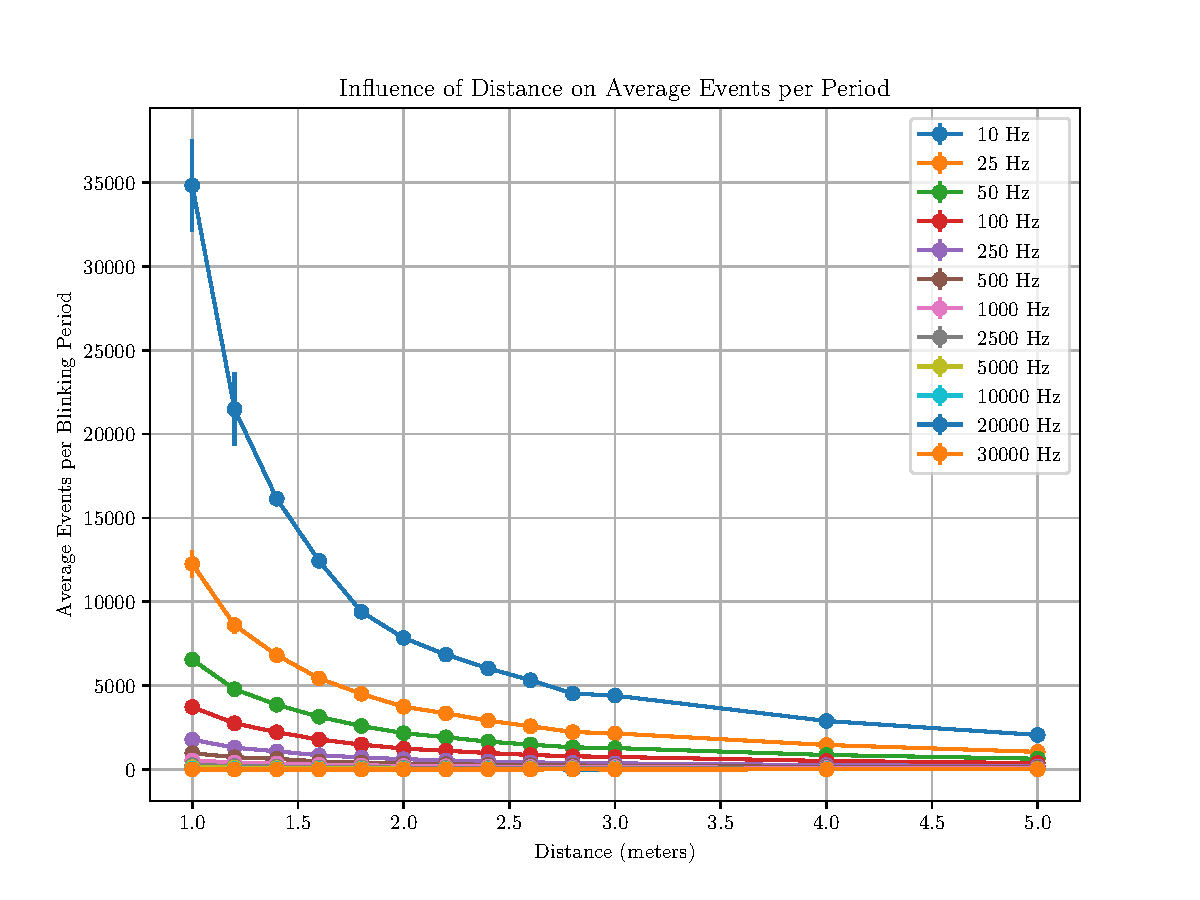
\includegraphics[width=0.5\textwidth]{./fig/semestral/dist.pdf}
	  \label{fig:dist_1}
	}
	\subfloat[Influence of distance on the log of average number of events.] {
	  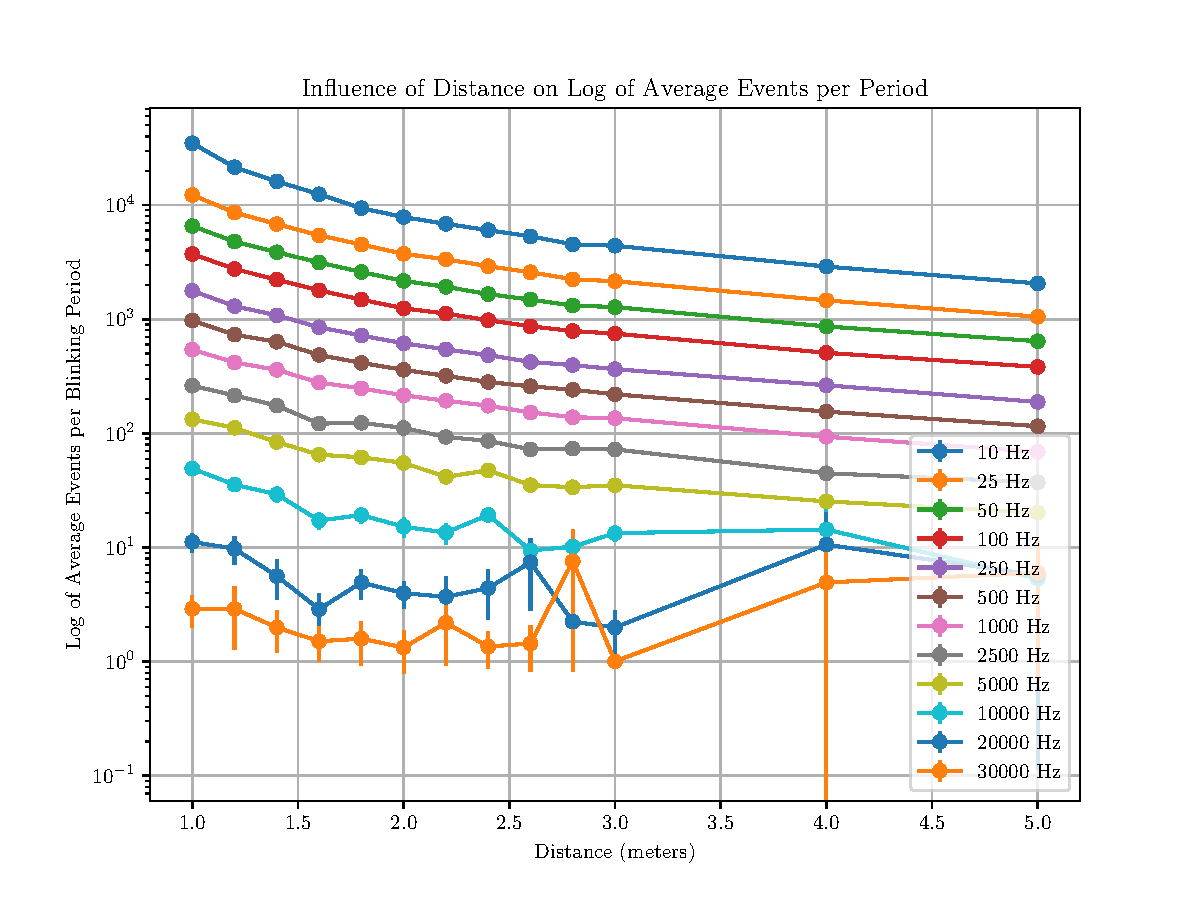
\includegraphics[width=0.5\textwidth]{./fig/semestral/distlog.pdf}
	  \label{fig:dist_2}
	}
	\caption{
  The influence of distance on the average number of events with the UAV rotated 0 degrees relative to the event camera on \reffig{fig:dist_1}, and with the log of the average number of events on \reffig{fig:dist_2}.
  }
	\label{fig:dist}
\end{figure}
\begin{figure}[H]
	\centering
	\subfloat[Influence of frequency on the average number of events.] {
	  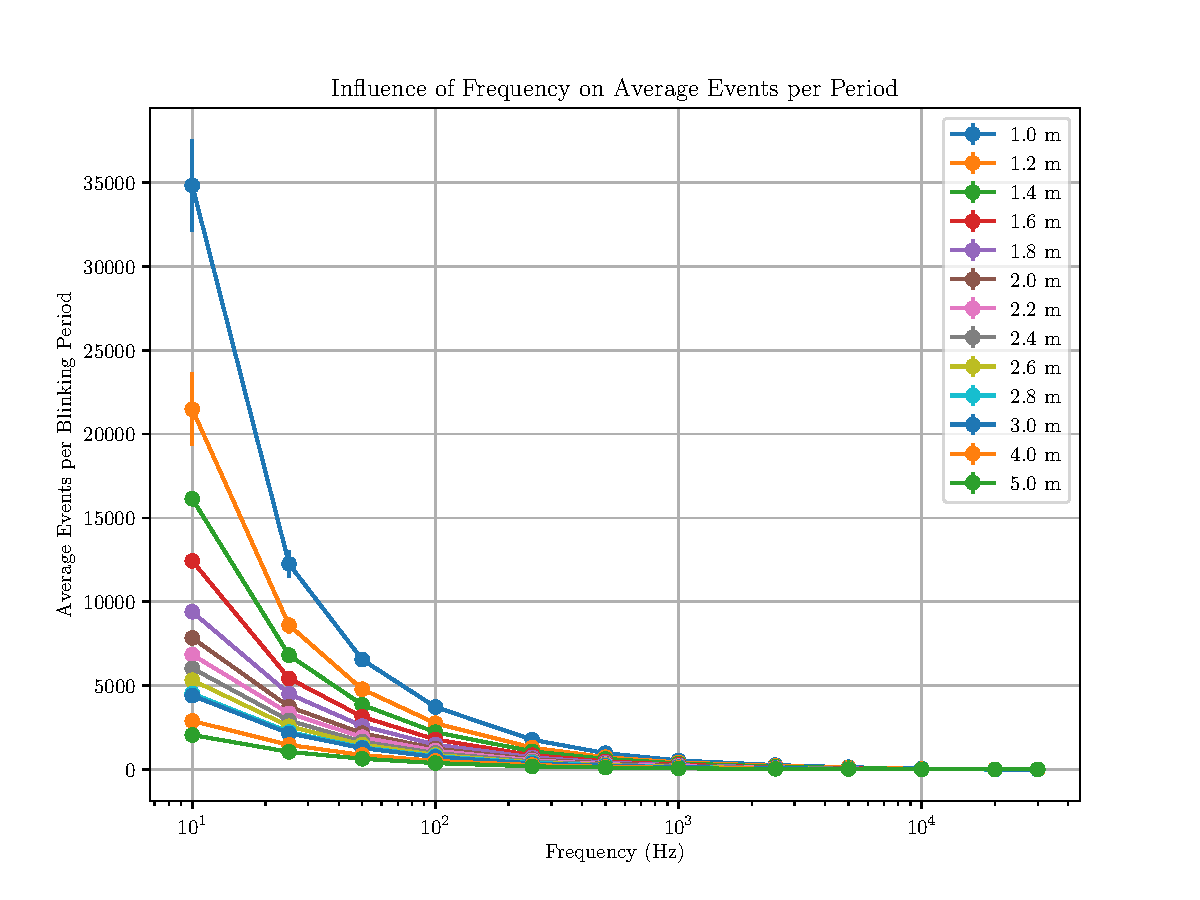
\includegraphics[width=0.5\textwidth]{./fig/semestral/freq.pdf}
	  \label{fig:freqs_1}
	}
	\subfloat[Influence of frequency on the log of average number of events.] {
	  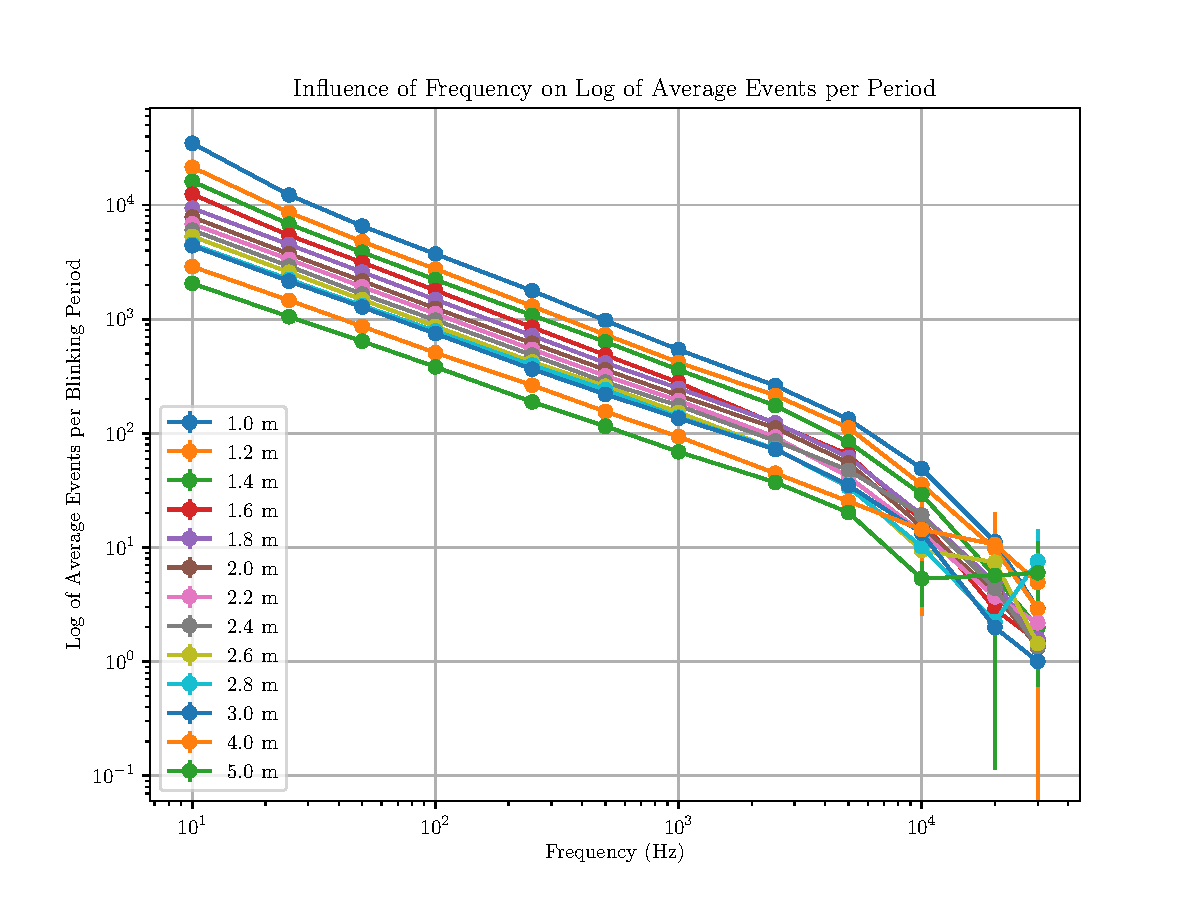
\includegraphics[width=0.5\textwidth]{./fig/semestral/freqlog.pdf}
	  \label{fig:freqs_2}
	}
	\caption{
  The influence of frequency on the average number of events with the UAV rotated 0 degrees relative to the event camera on \reffig{fig:freqs_1}, and with the log of the average number of events on \reffig{fig:freqs_2}.
  }
	\label{fig:freqs}
\end{figure}

\begin{figure}[H]
	\centering
	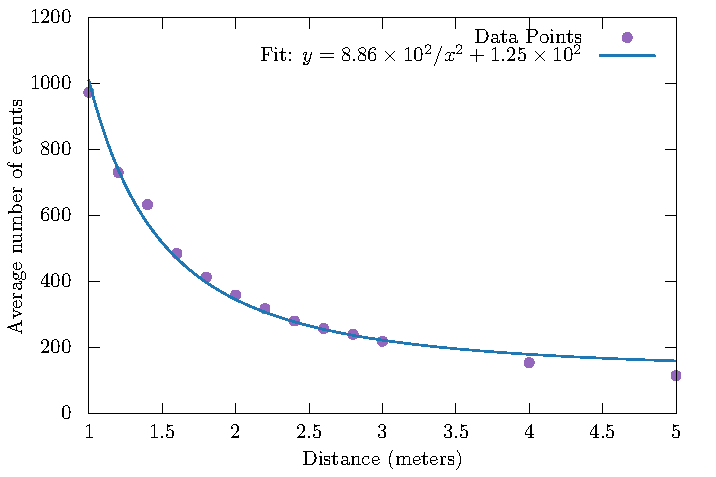
\includegraphics[width=0.90\textwidth]{./fig/semestral/inverse_square/square.pdf}
	\caption{Influence of distance data fitted with various curves.}
	\label{fig:fit1}
\end{figure}
More complex functions could be used to fit the data, but they would likely lead to overfitting rather than capturing the underlying trend in a generalizable way.
The inverse square law provides a relatively good approximation of the data.

\subsection{Rotation angle influence}
From the manufacturers datasheet for the UV LEDs\footnote{The datasheet of ProLight PM2B-1LLE 1W UV Power LED can be obtained from \url{https://www.tme.eu/Document/9dfb498784ffdd07892a42f4f17c6f37/PM2B-1LLE-DTE.pdf}}
used in the UVDAR system, we can learn that the LEDs have a Lambertian radiation pattern,
which can be seen on \reffig{fig:lambertian}.
\begin {figure}[H]
	\centering
	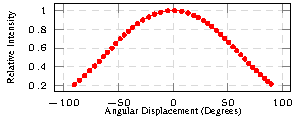
\includegraphics[width=0.75\textwidth]{./fig/semestral/lambertian/lambertian.pdf}
	\caption{Lambertian radiation pattern of the UV LED.}
	\label{fig:lambertian}
\end{figure}

This means that the intensity of the light emitted from the LED decreases with the cosine
of the angle between the normal of the LED and the direction of the light \refeq{eq:lambertian}.
\begin{equation}
	I(\theta) = I_0\cos(\theta)
	\label{eq:lambertian}
\end{equation}
If we shift those distributions by $\pm 45$ degrees and sum them together, we can see the
theoretical distribution of the light emmited from the singular UAV arm \reffig{fig:lambert_combined}.
\begin {figure}[H]
	\centering
	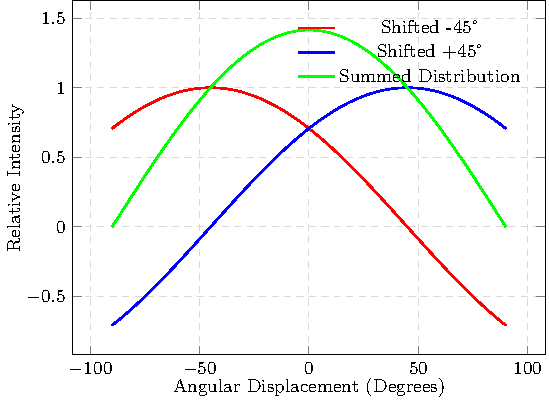
\includegraphics[width=0.50\textwidth]{./fig/semestral/lambertian/3lambertian.pdf}
	\caption{Radiation pattern of two lambertian light sources shifted by $\pm 45$ degrees.}
	\label{fig:lambert_combined}
\end{figure}
With the dataset of the rotation of the UAV relative to the camera we will get the following results
on \reffig{fig:angles}.

\begin{figure}[H]
	\centering
	\subfloat[Influence of rotation of the UAV on the log of average number of events at 0.5 m.] {
	  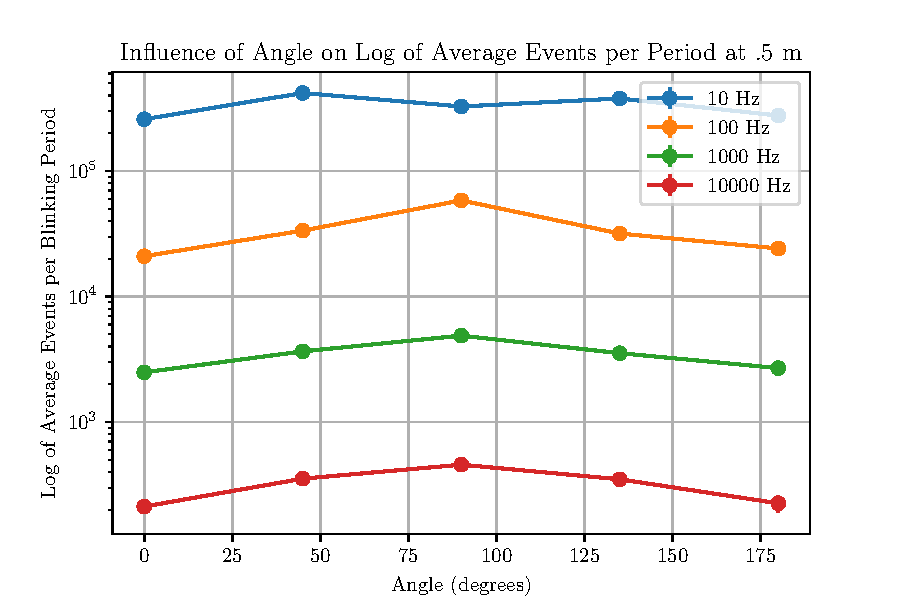
\includegraphics[width=0.5\textwidth]{./fig/semestral/angle1.pdf}
	  \label{fig:angle_1}
	}
	% \subfloat[Influence of rotation of the UAV on the log of average number of events at 1 m.] {
	%   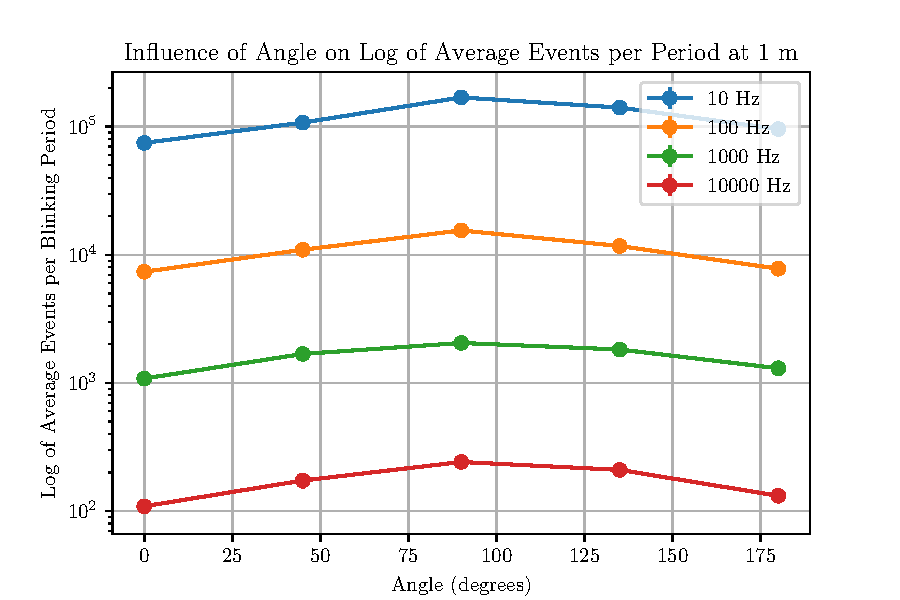
\includegraphics[width=0.5\textwidth]{./fig/semestral/angle2.pdf}
	%   \label{fig:angle_2}
	% }
	\subfloat[Influence of rotation of the UAV on the log of average number of events at 2 m.] {
	  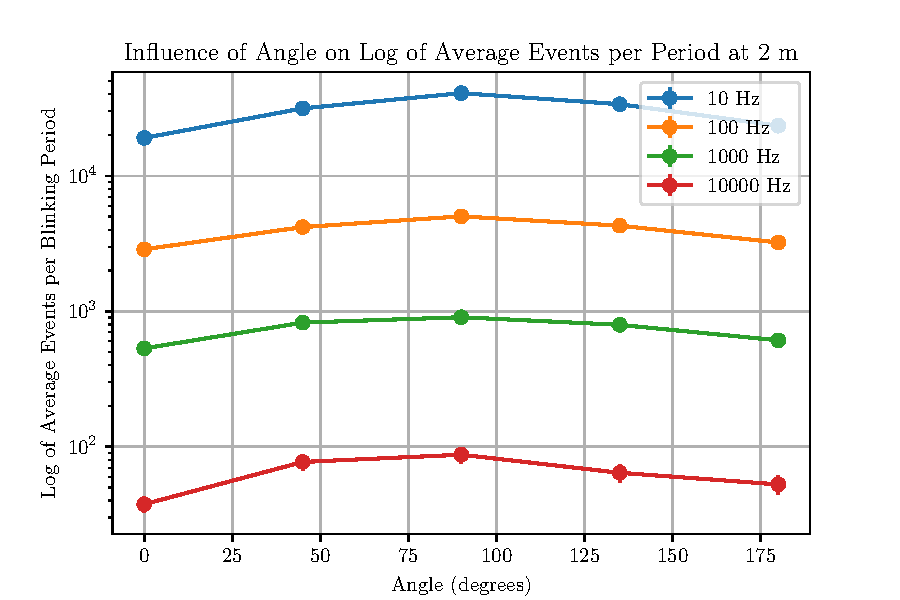
\includegraphics[width=0.5\textwidth]{./fig/semestral/angle3.pdf}
	  \label{fig:angle_3}
	}
	\caption{
  The influence of rotation angle on the log of average number of events at 0.5 m on \reffig{fig:angle_1} and at 2 m on \reffig{fig:angle_3}.
  }
	\label{fig:angles}
\end{figure}
The data show a rough approximation of the theoretical distribution on \reffig{fig:lambert_combined},
but with a drop of intensity at the middle of the distribution. This could be caused
by the fact that LEDs, when close to the camera, can be perceived as multiple light sources,
but when moved further away, they merge into one source as shown on \reffig{fig:leds}.

\begin{figure}[H]
	\centering
	\subfloat[2 LEDs with blinking frequency of 10 Hz at 0.5 m.] {
	  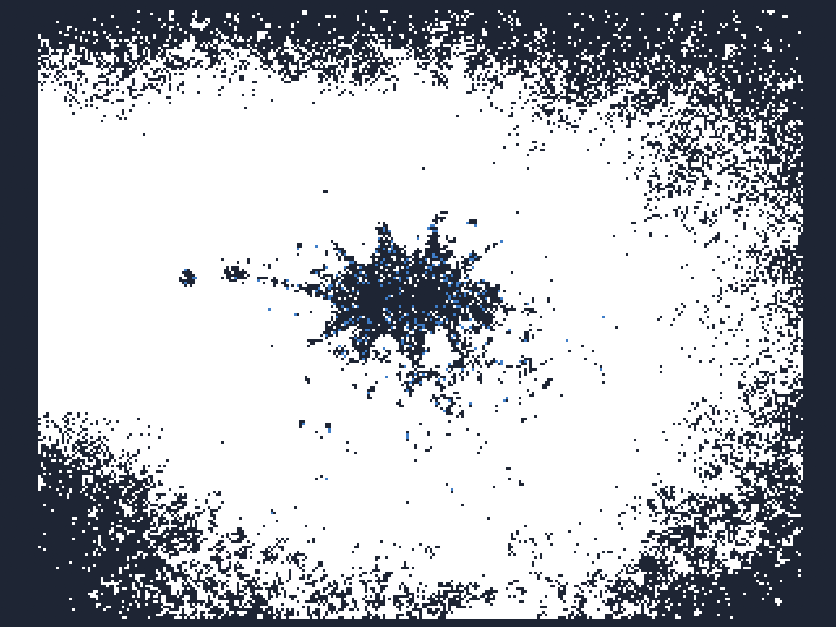
\includegraphics[width=0.5\textwidth]{./fig/photos/2leds_05m.png}
	  \label{fig:leds_1}
	}
	\subfloat[2 LEDs with blinking frequency of 10 Hz at 2 m.] {
	  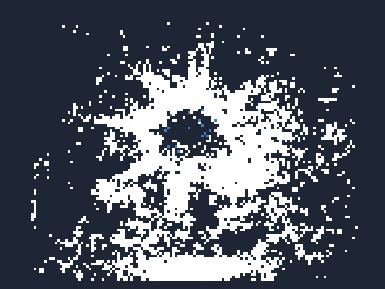
\includegraphics[width=0.5\textwidth]{./fig/photos/2leds_2m.png}
	  \label{fig:leds_2}
	}
	\caption{
  The light source on one arm of the UAV, consisting of two UV LEDs, blinking at a frequency of 10 Hz,
  placed at 0.5 m on \reffig{fig:leds_1} and 2 m at \reffig{fig:leds_2}.
  }
	\label{fig:leds}
\end{figure}
What we can also observe from \reffig{fig:leds} are the star-like shapes of the LEDs, which are supposed to be circular.
Those shapes are caused by light diffraction (and are named diffraction spikes), which are, in turn, caused by the aperture
blades in the lens of the camera. The number
of star spikes depend on the number of blades, the set aperture and the light source intensity then causes stars of different
levels of profoundness.\cite{lendermann2018computational} We can observe this by comparing how profound the star shapes are on different
frequencies, as shown on \reffig{fig:stars}.

\begin{figure}[H]
	\centering
	\subfloat[LED blinking at 10 Hz at 1.0 m] {
	  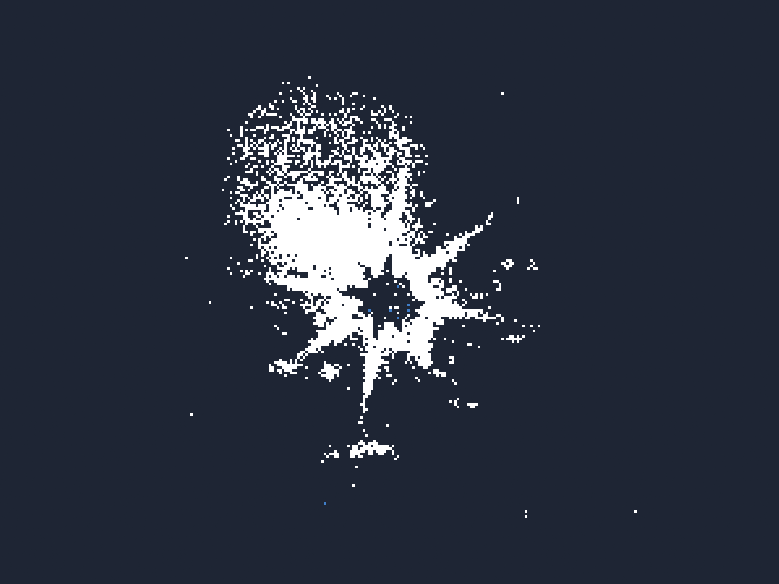
\includegraphics[width=0.5\textwidth]{./fig/photos/led_10hz.png}
	  \label{fig:stars_1}
	}
	\subfloat[LED blinking at 1 kHz at 1.0 m] {
	  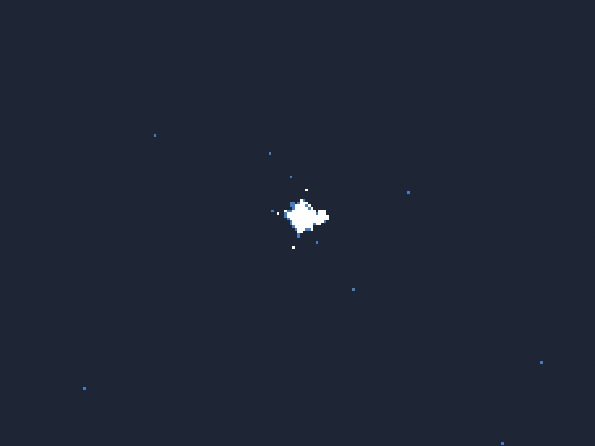
\includegraphics[width=0.5\textwidth]{./fig/photos/led_1000hz.png}
	  \label{fig:stars_2}
	}
	\caption{
  Two same LED light sources at 1.0 meters, blinking at 10 Hz and 1 kHz.
  \reffig{fig:stars_1} shows a visible diffraction star (while being much brighter), while \reffig{fig:stars_2} shows a
  much more cicular source of light that is not as bright.
  }
	\label{fig:stars}
\end{figure}